\section{An archived shared-memory probe in historical context}
\label{sec:probe}
This appendix reanalyzes an existing exploratory prototype, separate from the
fresh TIDE kernel and the literature evidence above. No simulations were
rerun for the review. The local record contains 140 output files: 20 baseline,
100 intervention, and 20 ownership-comparison files. Ten ownership-comparison
cases repeat an earlier condition, leaving 130 distinct seed/configuration
tuples. The source and raw outputs remain local; the review bundle includes
the ten plotted records, their source filenames and SHA-256 hashes, and the
extraction and plotting scripts.

\subsection{What the recorded comparison establishes}
The probe uses a $48\times48$ torus, 32 bytes per site, separate execution
pointers, and a supplied 17-byte ancestor. Updates run sequentially in CPU
birth order, four instructions per CPU per round; this is not TIDE's chosen
two-phase default. Figure~\ref{fig:probe} compares unrestricted and claimed
writes under one shared setting: local removal above one CPU per site,
maximum age 200 rounds, successful-write coverage before spawn, and per-byte
copy mutation 0.003. All five seeds per condition are shown.

\begin{figure}[!htbp]
\centering
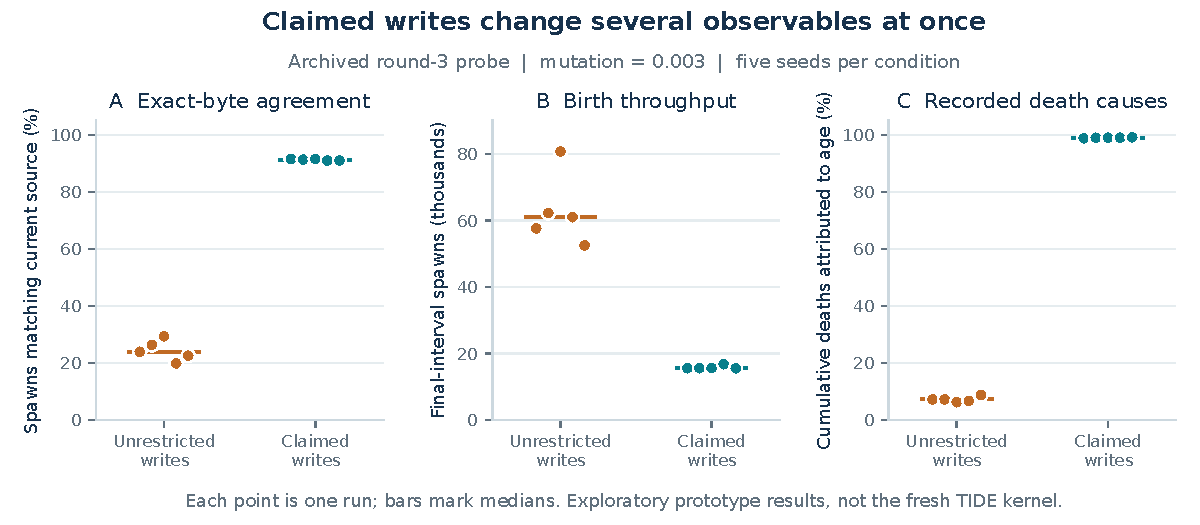
\includegraphics[width=\textwidth]{figures/probe-tradeoffs.pdf}
\caption{Reanalysis of archived round-3 prototype outputs, not a literature
figure or fresh TIDE result. Each point is one seed; horizontal bars are
medians, not confidence intervals. A compares target bytes with the executing
CPU's current memory site at spawn; it does not measure functional heredity.
A and B use the last 2,000-round interval of 20,000-round runs; C uses
cumulative death counters. Claimed writes jointly change body protection,
allocation ownership, vacancy access, and transfer rules, so this is a bundled
intervention. Values are read from the original logs; byte percentages retain
their original two-decimal rounding.}
\label{fig:probe}
\end{figure}

Under mutation, claimed writes raise final byte agreement from approximately
20--29\% to 91--92\%, while reducing final birth throughput by 3.38--5.17 times
for the same seed identifiers. The random-event histories need not remain
coupled across these treatments. Almost all recorded deaths under claimed
writes are attributed to age; most under unrestricted writes are local-cap
removals after arrivals by birth or movement. Overwriting bytes itself does
not remove a CPU in this implementation. The plot therefore supports a change
in several recorded observables, not a demonstrated gain in evolutionary
capacity or the isolated effect of body protection.

\subsection{How earlier systems addressed the same questions}
\textbf{Construction before new execution.}
Tierra's later V5.0 manual explicitly motivates a movement-count threshold
before division by the production of empty offspring when it is absent
\citep{RayManual1998}. Repeated writes to one address can satisfy its documented
count; this differs from the probe's distinct-offset coverage. The manual's
two descriptions disagree about the size denominator, so the exact threshold
requires version-specific code inspection. Avida separately checks allocation,
size, executed-parent fraction, and copied-offspring fraction before division
\citep{OfriaWilke2004}. Its main text and appendix also give different fractions.
The transferable distinction is between reservation, construction evidence,
and reproductive viability, not a universal numerical gate.

\textbf{Population survival after reproduction fails.}
Avida's authors explicitly warn that birth-only replacement can leave a
population present after self-replication is lost, and describe optional
death after a number of executed instructions \citep{OfriaWilke2004}.
Coreworld/Venus instead limits execution through local renewable resources;
resource failure and certain instructions remove pointers, while other rules
inject them \citep{Rasmussen1991}. Spatial Stringmol has stochastic decay and
vacancy-dependent product placement, yet still reports extinctions
\citep{Hickinbotham2021}. These are different turnover processes. An independent
death clock can reveal reproductive failure rather than rescue the population.

\textbf{Overwrite and interaction.}
Coreworld's authors report seeded replicators losing their reproductive
organization through noise and mutual overwriting \citep{Rasmussen1991}.
Tierra protects body and daughter-memory writes while permitting foreign
execution \citep{Ray1991}. This is a historical architectural contrast, not a
controlled demonstration that ownership is necessary. For functional diagnosis,
Avida tests descendant viability and Stringmol replays mutation-free reactions
in both orientations \citep{OfriaWilke2004,Hickinbotham2021}. The latter procedure
is particularly useful when solitary viability would miss partner dependence.

\subsection{Corrections and discriminating next controls}
The source audit narrows several initial interpretations. Baseline freezes
occur with 1,024 CPUs on 2,304 sites, so full occupancy is not necessary.
Successful-write coverage records historical writes, not the final integrity
or provenance of the destination. A count of surviving CPUs that previously
spawned is not the interval birth count. Memory-string richness includes
relics and allocations. Finally, the stored digest omits RNG state, ages,
coverage masks, and other future-relevant fields; matching recorded digests
does not establish full-state deterministic replay.

The next controls should separate three questions: whether division requires
reservation, counted writing, or distinct-address coverage; whether turnover
continues when births are suppressed; and whether body protection or
single-writer allocation causes the observed throughput change. Mutation-free
descendant and partner replay should accompany byte metrics. These are
proposed experiments, not changes to the agreed kernel contract. The detailed
source comparison and audit remain in the repository's research notes.
